% 4. Versuchsauswertung

\chapter{Auswertung und Diskussion}
\label{chap:versuchsauswertung}

\section{Aufnahme einer Münze}
Begonnen wurde der Versuch mit der Aufnahme einer Kupfermünze, in diese wurden zwei Löcher gebohrt, wobei eines mit einem anderen Material wieder gefüllt worden ist. Mithilfe dieser Probe sollten die Funktion des REM sowie verschiedene Einstellungsmöglichkeiten erkundet werden.\\

Als erstes wurde der Everhart-Thronley-Detektor im SE und RE Modus (SEI) verwendet und dabei die Beschleunigungsspannung variiert.
\begin{figure}[h]
    \centering
    
    \begin{subfigure}[b]{0.25\textwidth}
        \centering
        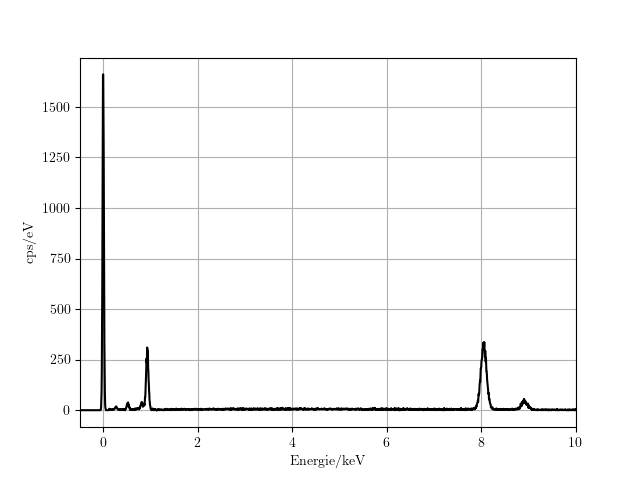
\includegraphics[width=\textwidth]{Auswertung/A/EdxFl.png}
        \caption{$U_B = 10$ kV}
    \end{subfigure}
    \hfill
    \begin{subfigure}[b]{0.25\textwidth}
        \centering
        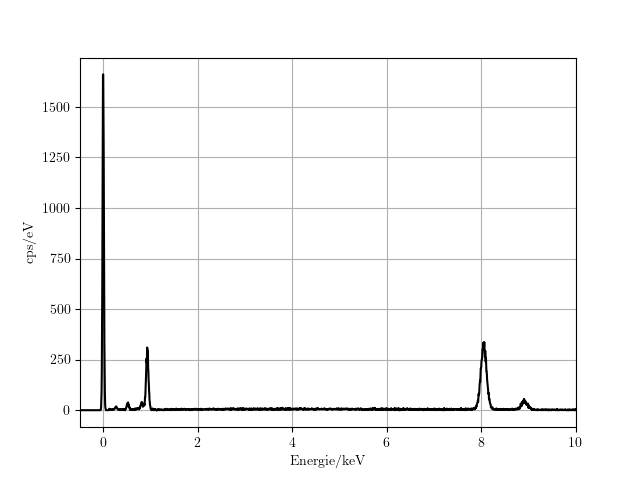
\includegraphics[width=\textwidth]{Auswertung/A/EdxFl.png}
        \caption{$U_B = 10$ kV}
    \end{subfigure}
\end{figure}